% Options for packages loaded elsewhere
\PassOptionsToPackage{unicode}{hyperref}
\PassOptionsToPackage{hyphens}{url}
\PassOptionsToPackage{dvipsnames,svgnames,x11names}{xcolor}
%
\documentclass[
  10pt,
  a4paper,
]{article}
\usepackage{amsmath,amssymb}
\usepackage{iftex}
\ifPDFTeX
  \usepackage[T1]{fontenc}
  \usepackage[utf8]{inputenc}
  \usepackage{textcomp} % provide euro and other symbols
\else % if luatex or xetex
  \usepackage{unicode-math} % this also loads fontspec
  \defaultfontfeatures{Scale=MatchLowercase}
  \defaultfontfeatures[\rmfamily]{Ligatures=TeX,Scale=1}
\fi
\usepackage{lmodern}
\ifPDFTeX\else
  % xetex/luatex font selection
\fi
% Use upquote if available, for straight quotes in verbatim environments
\IfFileExists{upquote.sty}{\usepackage{upquote}}{}
\IfFileExists{microtype.sty}{% use microtype if available
  \usepackage[]{microtype}
  \UseMicrotypeSet[protrusion]{basicmath} % disable protrusion for tt fonts
}{}
\makeatletter
\@ifundefined{KOMAClassName}{% if non-KOMA class
  \IfFileExists{parskip.sty}{%
    \usepackage{parskip}
  }{% else
    \setlength{\parindent}{0pt}
    \setlength{\parskip}{6pt plus 2pt minus 1pt}}
}{% if KOMA class
  \KOMAoptions{parskip=half}}
\makeatother
\usepackage{xcolor}
\usepackage[margin=21mm]{geometry}
\usepackage{longtable,booktabs,array}
\usepackage{calc} % for calculating minipage widths
% Correct order of tables after \paragraph or \subparagraph
\usepackage{etoolbox}
\makeatletter
\patchcmd\longtable{\par}{\if@noskipsec\mbox{}\fi\par}{}{}
\makeatother
% Allow footnotes in longtable head/foot
\IfFileExists{footnotehyper.sty}{\usepackage{footnotehyper}}{\usepackage{footnote}}
\makesavenoteenv{longtable}
\usepackage{graphicx}
\makeatletter
\def\maxwidth{\ifdim\Gin@nat@width>\linewidth\linewidth\else\Gin@nat@width\fi}
\def\maxheight{\ifdim\Gin@nat@height>\textheight\textheight\else\Gin@nat@height\fi}
\makeatother
% Scale images if necessary, so that they will not overflow the page
% margins by default, and it is still possible to overwrite the defaults
% using explicit options in \includegraphics[width, height, ...]{}
\setkeys{Gin}{width=\maxwidth,height=\maxheight,keepaspectratio}
% Set default figure placement to htbp
\makeatletter
\def\fps@figure{htbp}
\makeatother
\setlength{\emergencystretch}{3em} % prevent overfull lines
\providecommand{\tightlist}{%
  \setlength{\itemsep}{0pt}\setlength{\parskip}{0pt}}
\setcounter{secnumdepth}{-\maxdimen} % remove section numbering
\usepackage{amsmath,amssymb,mathtools}
\usepackage{fontspec}
\usepackage{unicode-math}
\setmainfont{Noto Serif}
\setsansfont{Noto Sans}
\setmonofont{DejaVu Sans Mono}[Scale=0.78]
\setmathfont{latinmodern-math.otf}
\usepackage{xurl}
\usepackage{fvextra}
\DefineVerbatimEnvironment{Highlighting}{Verbatim}{breaklines,commandchars=\\\{\}}
\usepackage{microtype}
\usepackage{fancyhdr}
\usepackage{etoolbox}
\usepackage{needspace}
\pagestyle{fancy}
\fancyhf{}
\fancyhead[L]{\footnotesize Research review edition}
\fancyhead[R]{\footnotesize 26 September 2026}
\fancyfoot[R]{\thepage}
\renewcommand{\headrulewidth}{0.3pt}
\setlength{\headheight}{14pt}
\setlength{\emergencystretch}{3em}
\setlength{\parskip}{5pt}
\setlength{\tabcolsep}{4pt}
\renewcommand{\arraystretch}{1.13}
\AtBeginEnvironment{longtable}{\footnotesize}
\AtBeginEnvironment{quote}{\small}
\allowdisplaybreaks
\makeatletter
\renewcommand\section{\@startsection{section}{1}{\z@}{-2.4ex \@plus -1ex \@minus -.2ex}{1.2ex \@plus .2ex}{\normalfont\Large\bfseries}}
\renewcommand\subsection{\@startsection{subsection}{2}{\z@}{-2ex \@plus -.8ex \@minus -.2ex}{.9ex \@plus .2ex}{\normalfont\large\bfseries}}
\makeatother
\ifLuaTeX
  \usepackage{selnolig}  % disable illegal ligatures
\fi
\usepackage{bookmark}
\IfFileExists{xurl.sty}{\usepackage{xurl}}{} % add URL line breaks if available
\urlstyle{same}
\hypersetup{
  colorlinks=true,
  linkcolor={Maroon},
  filecolor={Maroon},
  citecolor={Blue},
  urlcolor={black},
  pdfcreator={LaTeX via pandoc}}

\author{}
\date{}

\begin{document}

\section{Post-injection pilot: executed
results}\label{post-injection-pilot-executed-results}

\subsection{Local readability, directional evidence and finite-window
limitations}\label{local-readability-directional-evidence-and-finite-window-limitations}

\textbf{Study ID: P01-ID1 \textbar{} Results log v1.2 \textbar{} 26
September 2026}

This is a results log, not another journal manuscript. It records one
specified computational pilot, its independent-method checks and its
limits. The primary model family and outcome were recorded before
execution. The sign tests, precision calculation and additional
window/eligibility diagnostics below were added after the outcome was
known; they are explicitly secondary reanalyses, not changes to the
original study. No external preregistration, human specialist review,
participant experiment or cosmological observation is claimed.

\subsection{1. Main result}\label{main-result}

The source was switched off after injection. The predeclared change
relative to matched frozen evolution was negative. A later factorial
extension asks a different question by comparing two Hamiltonian
orientations at fixed injection; its paired contrast is positive.
Neither number replaces the other. At six qubits with rotated injection,
the mean normalized change was \textbf{-0.015225}, with 68 negative and
28 positive unit-level contrasts. None of the 96 primary units produced
a new singleton record satisfying the strict initial-information floor
and error threshold throughout any declared half-unit window, in either
frame.

The full source bit was not erased: the two global conditional states
remained orthogonal under their shared unitary. Local access, transfer,
redundancy and global information are different outcomes. There is no
inference here that AIU or a general locality-record law is false.

\subsection{2. Exactly what ran}\label{exactly-what-ran}

There are \textbf{192 independent model/circuit units}, 96 at four
qubits and 96 at six qubits. Each unit has two paired injection arms,
giving \textbf{384 arm evaluations}, not 384 independent samples. Each
arm is evaluated in two frames over 101 checkpoints. The primary
statistic uses 50 positive-time checkpoints fixed before execution. The
paired off-evolution control is analytic identity evolution, not a
separately random sample.

The internal model is a random anisotropic nearest-neighbour Pauli chain
with independent fields. It differs from an earlier review proposal that
varied the amplitude of one fixed Hamiltonian shape. The alternate frame
is an independent depth-two adjacent-pair Haar circuit. The graph and
allowable readout algebras are supplied. Randomized coefficients do not
make this a representative sample of all physical systems.

The executable simulation uses full finite-dimensional state vectors,
not a quantum device. Runtime of the main numerical solve in this
environment was approximately 2.08 seconds; that excludes writing,
derivation, source checking and verification and is not a portable
performance guarantee.

\subsection{3. Primary and sensitivity
results}\label{primary-and-sensitivity-results}

\Needspace{12\baselineskip}

\textbf{Table 1. Baseline-subtracted local-readability contrast}

\begin{longtable}[]{@{}
  >{\raggedright\arraybackslash}p{(\columnwidth - 8\tabcolsep) * \real{0.2000}}
  >{\raggedright\arraybackslash}p{(\columnwidth - 8\tabcolsep) * \real{0.2000}}
  >{\raggedright\arraybackslash}p{(\columnwidth - 8\tabcolsep) * \real{0.2000}}
  >{\raggedright\arraybackslash}p{(\columnwidth - 8\tabcolsep) * \real{0.2000}}
  >{\raggedright\arraybackslash}p{(\columnwidth - 8\tabcolsep) * \real{0.2000}}@{}}
\toprule\noalign{}
\begin{minipage}[b]{\linewidth}\raggedright
Qubits
\end{minipage} & \begin{minipage}[b]{\linewidth}\raggedright
Injection arm
\end{minipage} & \begin{minipage}[b]{\linewidth}\raggedright
Mean z
\end{minipage} & \begin{minipage}[b]{\linewidth}\raggedright
Approximate bootstrap 95\% interval
\end{minipage} & \begin{minipage}[b]{\linewidth}\raggedright
Positive / negative / tie
\end{minipage} \\
\midrule\noalign{}
\endhead
\bottomrule\noalign{}
\endlastfoot
4 & native & 0.015125 & {[}0.008577, 0.022237{]} & 61 / 35 / 0 \\
4 & rotated & -0.028761 & {[}-0.035284, -0.022440{]} & 18 / 78 / 0 \\
6 & native & 0.011674 & {[}0.007238, 0.016167{]} & 65 / 31 / 0 \\
6 & rotated & -0.015225 & {[}-0.021070, -0.009646{]} & 28 / 68 / 0 \\
\end{longtable}

Only the six-qubit rotated arm is primary. The native-injection arm
compares its native frame against the paired alternate frame, which is
not its own physical injection frame. Do not pool the four rows as
independent confirmations.

For the primary row, the distribution-free Hoeffding 95\% interval is
\textbf{{[}-0.292446, 0.261996{]}}. It crosses zero. The much narrower
bootstrap interval is approximate and informative about this finite
empirical distribution; it is not a distribution-free guarantee or a
confirmation of a universal negative sign. This original sample does not
support a positive value of its own target. It cannot isolate the effect
of changing the dynamics-locality frame, which it held fixed.

\par\medskip\noindent\begin{minipage}{\linewidth}

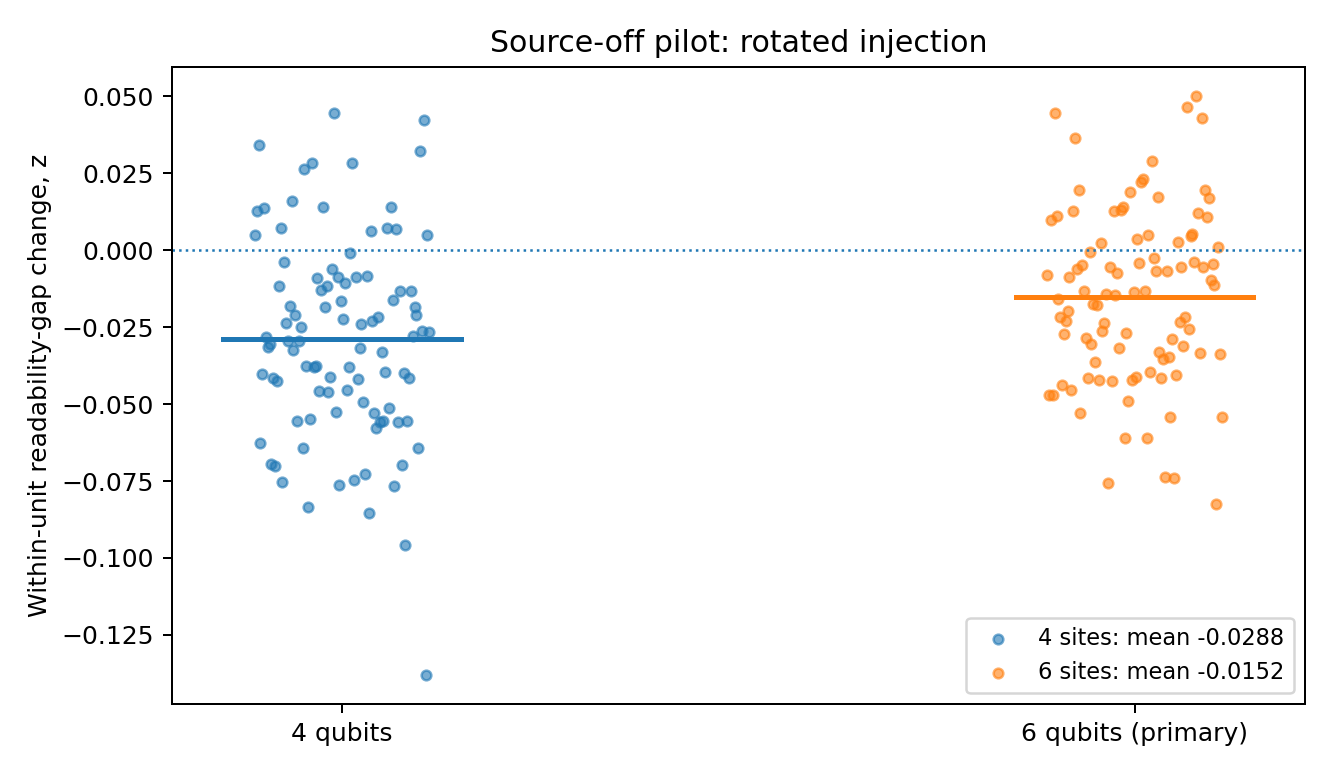
\includegraphics{../../figures/pilot_contrast_distribution.png}

\textbf{Figure 1. Each point is one independent model unit. Zero is no
change in the readability gap relative to the no-evolution baseline.
This is not a probability of AIU or a test of the older LRA-count
margin.}

\end{minipage}\par\medskip

\subsubsection{3.1 A negative change does not mean C has better absolute
readout}\label{a-negative-change-does-not-mean-c-has-better-absolute-readout}

For the six-qubit rotated arm, mean singleton trace distance at
switch-off was approximately \textbf{0.208408 in L} and \textbf{0.166667
in C}. The corresponding post-time averages were \textbf{0.197702 in L}
and \textbf{0.186411 in C}. Thus L's initial gap of \textbf{0.041742}
narrowed to \textbf{0.011292}. Half that gap change is the negative
primary result. Claiming that records migrated to C would overstate this
statistic.

A scrambled representation can spread partial distinguishing information
over multiple sites; sums of singleton distances are not additive global
information. The primary mean therefore measures accessibility, not
independent bits, redundant strong records or a unique preferred
subsystem structure.

\par\medskip\noindent\begin{minipage}{\linewidth}

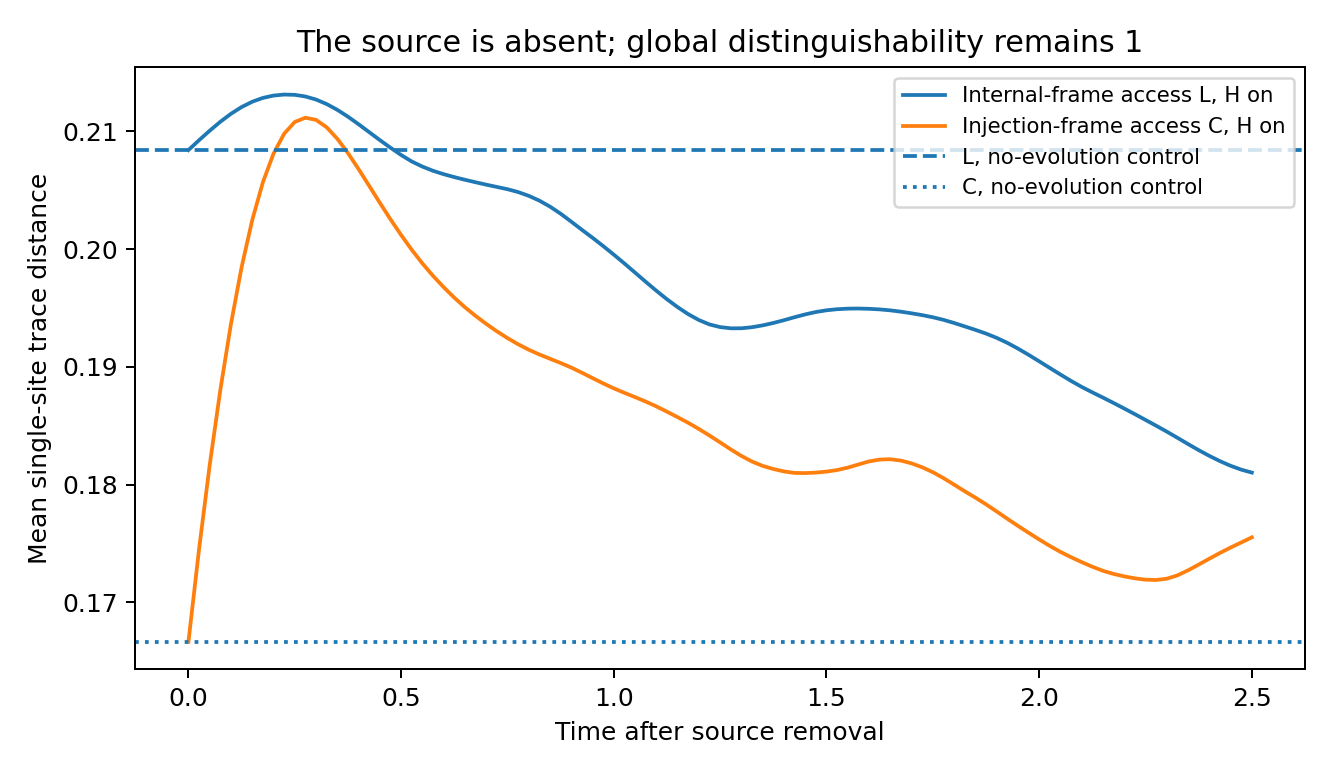
\includegraphics{../../figures/pilot_readability_curves.png}

\textbf{Figure 2. Six-qubit rotated injection, means across 96 units.
The pulse ends at t=0; the source is absent thereafter. Horizontal
baselines are the matched frozen states. Weak local readability can
change even when no new fragment meets the strict record criterion.}

\end{minipage}\par\medskip

\subsubsection{3.2 Post hoc directional
analysis}\label{post-hoc-directional-analysis}

Let \(p_{\mathrm{pos}}\) be the probability of a positive nonzero unit
contrast. The exact sign test evaluates \(H_0:p_{\mathrm{pos}}=1/2\)
with independent signs. It does not assume symmetry of the full contrast
distribution, but independence alone is not the null. It is not a test
of zero mean. Ties use the original \(10^{-12}\) reporting tolerance;
none occur, and the smallest absolute contrast across these data is
greater than \(2.5\times10^{-4}\).

\Needspace{12\baselineskip}

\textbf{Table 2. Post hoc two-sided binomial sign tests}

\begin{longtable}[]{@{}
  >{\raggedright\arraybackslash}p{(\columnwidth - 6\tabcolsep) * \real{0.2500}}
  >{\raggedright\arraybackslash}p{(\columnwidth - 6\tabcolsep) * \real{0.2500}}
  >{\raggedright\arraybackslash}p{(\columnwidth - 6\tabcolsep) * \real{0.2500}}
  >{\raggedright\arraybackslash}p{(\columnwidth - 6\tabcolsep) * \real{0.2500}}@{}}
\toprule\noalign{}
\begin{minipage}[b]{\linewidth}\raggedright
Qubits / arm
\end{minipage} & \begin{minipage}[b]{\linewidth}\raggedright
Positive / negative
\end{minipage} & \begin{minipage}[b]{\linewidth}\raggedright
Unadjusted p
\end{minipage} & \begin{minipage}[b]{\linewidth}\raggedright
Holm-adjusted p, four-row family
\end{minipage} \\
\midrule\noalign{}
\endhead
\bottomrule\noalign{}
\endlastfoot
4 / native & 61 / 35 & 0.0103459 & 0.0103459 \\
4 / rotated & 18 / 78 & 4.44694e-10 & 1.77877e-9 \\
6 / native & 65 / 31 & 0.000674719 & 0.00134944 \\
6 / rotated & 28 / 68 & 0.0000545915 & 0.000163775 \\
\end{longtable}

The adjustment covers these four tests and does not require independence
between the paired arms. It does not account for unrestricted post hoc
exploration outside this stated family. Within the explicit sampling
law, the rotated-arm signs provide strong secondary evidence against
directional balance. This neither makes the mean a distribution-free
finding nor overturns the formal distinction between the executed
readability target and the older LRA hypotheses. The predeclared
bootstrap interval already provided approximate evidence about the mean;
it was not an empty or wholly inconclusive result.

\subsubsection{3.3 Precision limitation, not a retrospective power
claim}\label{precision-limitation-not-a-retrospective-power-claim}

At 96 units, the chosen range-only Hoeffding half-width is 0.277221.
Solving \(\sqrt{2\log(40)/N}\le0.015\) gives \(N\ge32791\). This is a
sufficient worst-case sample count for that confidence-interval
precision, not a minimum sample size required by every valid method and
not a power calculation. The width is much larger than the observed
effect. The pre-execution plan should have stated this limitation, and
the original plan is preserved without retrospective amendment. Future
studies should distinguish a justified precision budget, an
alternative-specific power analysis and computational feasibility. This
calculation is not a recommendation to run 32,791 units.

\subsection{4. Strict new-record
criterion}\label{strict-new-record-criterion}

The criterion required initial error at least 0.4999 and subsequent
error at most 0.1 throughout {[}0.5,1.0{]}, {[}1.0,1.5{]}, {[}1.5,2.0{]}
or {[}2.0,2.5{]}. At both sizes and in both arms, every possible upper
count for a new singleton record was zero in every window. Here that was
not an unequal-certificate problem: the initial-information floor or a
failing checkpoint already ruled out the strict condition numerically.
The raw data retain all cases.

This says nothing about larger fragments, looser tolerances, other
windows, different preparation laws or other Hamiltonians. Those would
be different analyses. They were not added after observing this outcome.
The numerical guard remains empirical rather than a formally certified
roundoff enclosure.

\subsubsection{4.1 What the zero count excludes, and what it does
not}\label{what-the-zero-count-excludes-and-what-it-does-not}

A review-stage diagnostic of the original stored trajectories separates
transient access from full-window persistence. In the native arm, 5
initially eligible site/unit pairs at four qubits and 10 at six qubits
briefly reached trace distance at least 0.8 at a positive-time
checkpoint. None satisfied a complete declared window. These are
site/unit pairs, not independent samples or counts of distinct systems;
they are not new strong persistent records. Thus the data themselves do
not support the general statement that internal dynamics cannot create
local source accessibility. In the rotated arm, none of the initially
eligible singletons reached this strict checkpoint threshold within the
recorded horizon.

Initial eligibility also differs between frames because partial source
information can already be distributed at switch-off. At six qubits with
rotated injection, 288 of 576 site/unit pairs are initially eligible in
L, compared with 480 in C. The definition deliberately asks about newly
informative fragments, so this difference is part of the target, not a
reason to remove inconvenient units. The companion mean-readability
statistic has a different denominator and remains unchanged. The full
diagnostic table is supplied in the supplement and data.

\subsection{5. Transport worked in the analytical
controls}\label{transport-worked-in-the-analytical-controls}

For the vacuum-versus-excitation encoding, the two-site exchange control
gives recipient distinguishability \(\sin^2 t\). At \(t=\pi/2\), the
source bit has transferred from the addressed site to its neighbour.
Four- and six-site exchange chains matched an independently evaluated
one-excitation hopping model. The sampled end-site distinguishability
reached approximately 0.972655 at time 2.80 for four sites and 0.911536
at time 3.95 for six sites. These are sampled control values, not
globally optimized arrival times or claims of new transport physics.

For a vacuum-versus-single-excitation code, let \(p_j(t)\) be the
excitation probability. Then \(d_j(t)=p_j(t)\) and \(\sum_j p_j(t)=1\).
Error at most 0.1 requires \(p_j\ge0.8\), so at most one singleton can
qualify at one time. This control demonstrates transport without high
redundant copying. It exposes why a redundancy measure is not
automatically a transport or geometry-recovery measure.

\par\medskip\noindent\begin{minipage}{\linewidth}

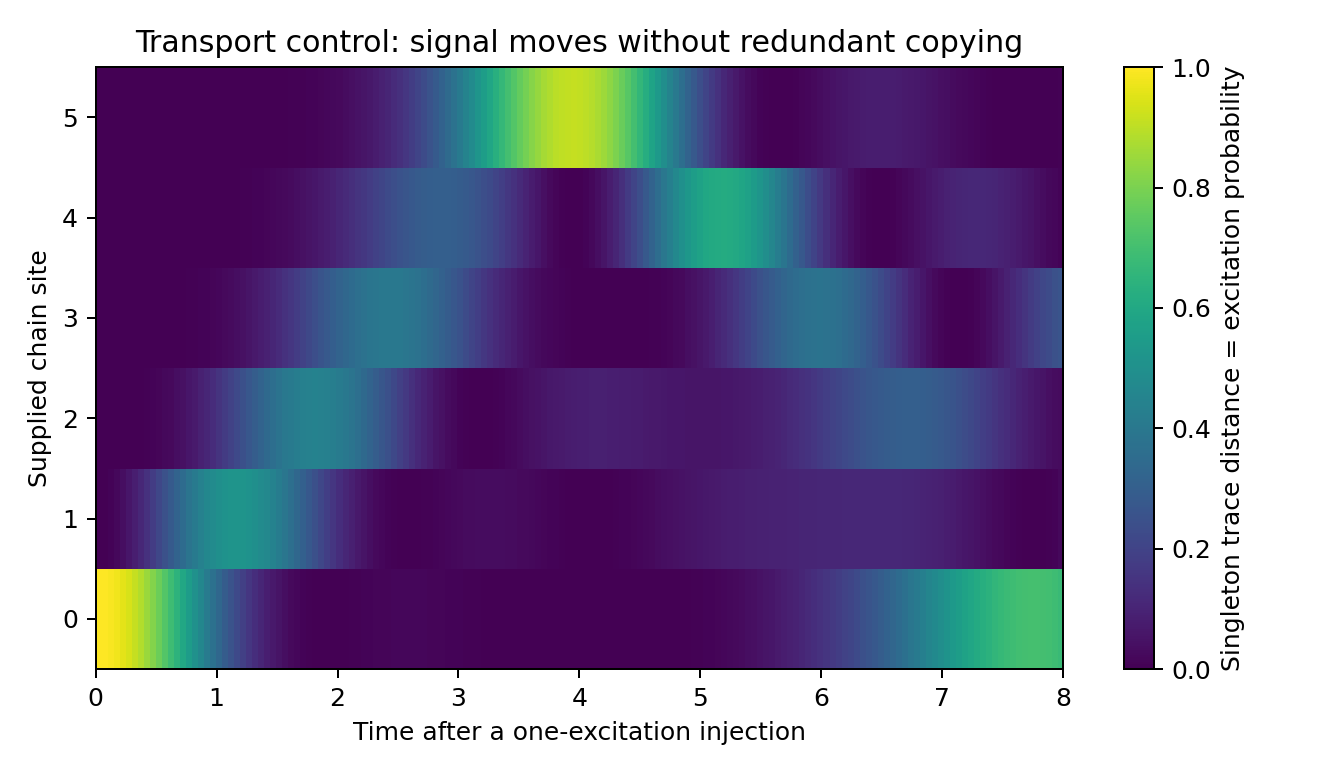
\includegraphics{../../figures/pilot_transport_control.png}

\textbf{Figure 3. Full-state calculation, independently matched to the
one-excitation reduction. Propagation is present although conservation
limits simultaneous strong singleton records. The chain and its
coordinates are supplied.}

\end{minipage}\par\medskip

\subsubsection{5.1 Transport-window and source-encoding
diagnostic}\label{transport-window-and-source-encoding-diagnostic}

The original windows end at 2.5. In the uniform exchange-chain control
using a vacuum-versus-excitation code, end-site distinguishability is
\(|f(t)|^2\). On the reviewer's 0.05 grid, it exceeds 0.8 during 2.4 to
3.2 at four sites and 3.6 to 4.3 at six sites. No complete declared
half-unit window lies inside either interval. This is a valid warning
that the windows cannot assess late far-end strong transfer in that
control.

The actual pilot uses opposite-phase superpositions of vacuum and a
single addressed excitation, not that control's source code. For the
ideal number-conserving exchange chain with the pilot code, direct
partial trace instead gives end-site distinguishability \(|f(t)|\). Its
qualification threshold corresponds to excitation probability 0.64, not
0.8. Both curves and their exact declared-window checks are supplied. No
complete original window passes at the far end for either encoding, but
the two threshold times must not be interchanged.

These controls do not establish that all zero counts in random
anisotropic chains were built in: those chains, their code, distances
and eligible fragments differ, and some near-site transient strong
signals were observed. The defensible conclusion is narrower: the strict
result is conditional on a restrictive floor, threshold and short
windows and cannot stand for absence of transport. No late-window rerun
or changed primary endpoint is included in this release.

\subsection{6. Verification}\label{verification}

A separate implementation does not import the main solver. It propagates
selected n=4 and n=6 units using exponential action and reduces full
density matrices rather than the main state-tensor shortcut. The largest
compared trace-distance discrepancy was \textbf{9.104e-15}. The largest
main-run norm error was \textbf{3.320e-14} and the largest branch
overlap magnitude \textbf{2.371e-14}.

The \textbf{36 checks passed}, with \textbf{0 failures}. These checks
include selected-trajectory agreement, zero evolution, identical
branches, passive conjugation, two-site transfer, one-excitation
conservation, closed stationary records and amplitude-damping erasure.
They are not 36 independent physical experiments. Numerical agreement is
not a formal floating-point proof.

A closed diagonal Hamiltonian preserves orthogonal product records
because their density matrices commute with H. Conversely, an ordinary
amplitude-damping channel reduces the distinguishability of
zero-versus-one states as \(e^{-t}\). These elementary controls correct
the overstatement that persistence always requires a large or
dissipative environment. What matters is the stated retention mechanism
and observable, not openness alone.

\subsection{7. Decision after the pilot}\label{decision-after-the-pilot}

\textbf{Keep the original result and the new counterfactual separate.}
The source-off pilot measures a change from frozen evolution with the
dynamics always native to L. Its negative mean is reproducible but is
not an isolated causal estimate of locality. The factorial extension
varies that dynamics frame at fixed injection and produces a positive
paired intervention contrast. It adds missing information rather than
changing the original question after the answer was seen.

This is not recovered locality: the frames, Hamiltonian family and
readout rules are all supplied. A named Lieb-Robinson mechanism has not
been identified merely by obtaining a positive scalar contrast. An
actual identification study would require multiple injections, a
reconstruction method not given its target and held-out prediction. An
open-system retention study separately needs a justified reservoir and
erasure controls. Neither extension is silently announced as completed
here.

\subsection{8. Reproduction and
provenance}\label{reproduction-and-provenance}

\nolinkurl{pilot/PRE_EXECUTION_PLAN.md}, \nolinkurl{pilot/config.json}
and \nolinkurl{pilot/PRE_EXECUTION_RECEIPT.json} retain the pre-outcome
specification and local hashes.
\nolinkurl{data/pilot_run/model_inputs.json} contains coefficients and
random-stream identifiers. \nolinkurl{trajectories_n4.npz} and
\nolinkurl{trajectories_n6.npz} contain raw per-site readability and
small validation examples. \nolinkurl{per_unit.json} retains the count
bounds and all individual outcomes.
\nolinkurl{code/run_injection_pilot.py} refuses a nonempty output
directory. The reviewer bundle includes the text, configuration and code
but omits binary trajectories to remain small.

No email was sent and no external review occurred. The specialist brief
accompanies \emph{Frame-Aligned Records} and its supplement for a later,
separately authorized circulation.

\subsection{9. Review-stage reimplementation and factorial
intervention}\label{review-stage-reimplementation-and-factorial-intervention}

\subsubsection{9.1 Same target, fresh
reimplementation}\label{same-target-fresh-reimplementation}

An independently written implementation supplied during review uses the
protocol's model law, 50 positive-time readouts, a two-layer
adjacent-pair Haar circuit and fresh seeds. Its author had to infer the
open-chain convention, the order \(U_C=L_2L_1\), and the leftmost
addressed site. Those inferred conventions were compared with the
original code, not certified by initial eligibility counts alone.
Matching a small diagnostic does not logically prove complete
implementation identity.

All supplied numerical summaries were re-executed with their stated
seeds. The six-qubit 60,000-unit rotated run gives mean -0.01412453 and
a range-only 95\% interval {[}-0.02521338, -0.00303568{]}. This is a new
sample from the explicit law, not a retrospective increase of the
original 96-unit sample. Its prediction file was supplied with a
matching hash; a local hash establishes integrity, not an externally
certified time of creation.

\subsubsection{9.2 The added factor and its
estimand}\label{the-added-factor-and-its-estimand}

For each paired unit, injection in L or C is crossed with dynamics
\(H_L=H\) or \(H_C=U_C H U_C^\dagger\). Readout remains in the same L
and C algebras. Let \(g_b^a\) be the post-time mean readability gap and
\(g_0^a\) its common initial gap at injection \(a\). Then

\[z_{ab}=\tfrac12(g_b^a-g_0^a),\qquad e_a=z_{aL}-z_{aC}=\tfrac12(g_L^a-g_C^a).\]

The baseline cancels in \(e_a\), so \(-1\le e_a\le1\). The factorial
contrast is not the old \(z_{CL}\), and a positive \(e_C\) need not make
either \(z_{CL}\) or \(z_{CC}\) positive. At six qubits the four means
are:

\begin{longtable}[]{@{}llll@{}}
\toprule\noalign{}
Injection & Dynamics L & Dynamics C & Difference \\
\midrule\noalign{}
\endhead
\bottomrule\noalign{}
\endlastfoot
L & 0.01400416 & 0.00349055 & 0.01051361 \\
C & -0.01402828 & -0.02666340 & 0.01263512 \\
\end{longtable}

The values were reproduced, not merely transcribed. The factorial code
originally retained aggregate JSON only. This replay additionally
retains per-unit z and before/after readability in NPZ arrays, with the
original seeds and input-generation code unchanged. It does not retain
every factorial state trajectory.

\subsubsection{9.3 Finite-family sampling
uncertainty}\label{finite-family-sampling-uncertainty}

The six disclosed contrasts cover two injection conditions at each of
four, six and eight qubits. The four- and six-qubit runs contain 20,000
independent model units per size; the eight-qubit run contains 1,000.
Four arms within one unit are paired, not four independent observations.
A simultaneous empirical-Bernstein bound uses the paired sample
variance, rescaling from {[}-1,1{]} and allocating error over both tails
and six targets {[}Maurer and Pontil 2009, Theorem 4{]}.

\begin{longtable}[]{@{}llll@{}}
\toprule\noalign{}
Qubits & Injection & Mean e & Simultaneous 95\% Bernstein interval \\
\midrule\noalign{}
\endhead
\bottomrule\noalign{}
\endlastfoot
4 & L & 0.005752 & {[}0.003528, 0.007976{]} \\
4 & C & 0.011074 & {[}0.008801, 0.013347{]} \\
6 & L & 0.010514 & {[}0.008604, 0.012423{]} \\
6 & C & 0.012635 & {[}0.010692, 0.014579{]} \\
8 & L & 0.010363 & {[}-0.020023, 0.040748{]} \\
8 & C & 0.012137 & {[}-0.018361, 0.042634{]} \\
\end{longtable}

This finite-sample result assumes iid units under the declared law and
faithful numerical evaluation. It makes no normal-distribution
assumption, but it does not account for unlimited undisclosed model
selection. The variance-sensitive analysis was specified during this
review, after the supplied summaries were known. It is a disclosed
secondary analysis, not a newly preregistered confirmatory study. The
older normal-approximation intervals and wider simultaneous Hoeffding
intervals are all retained in the CSV, not selected according to which
exclude zero.

\par\medskip\noindent\begin{minipage}{\linewidth}

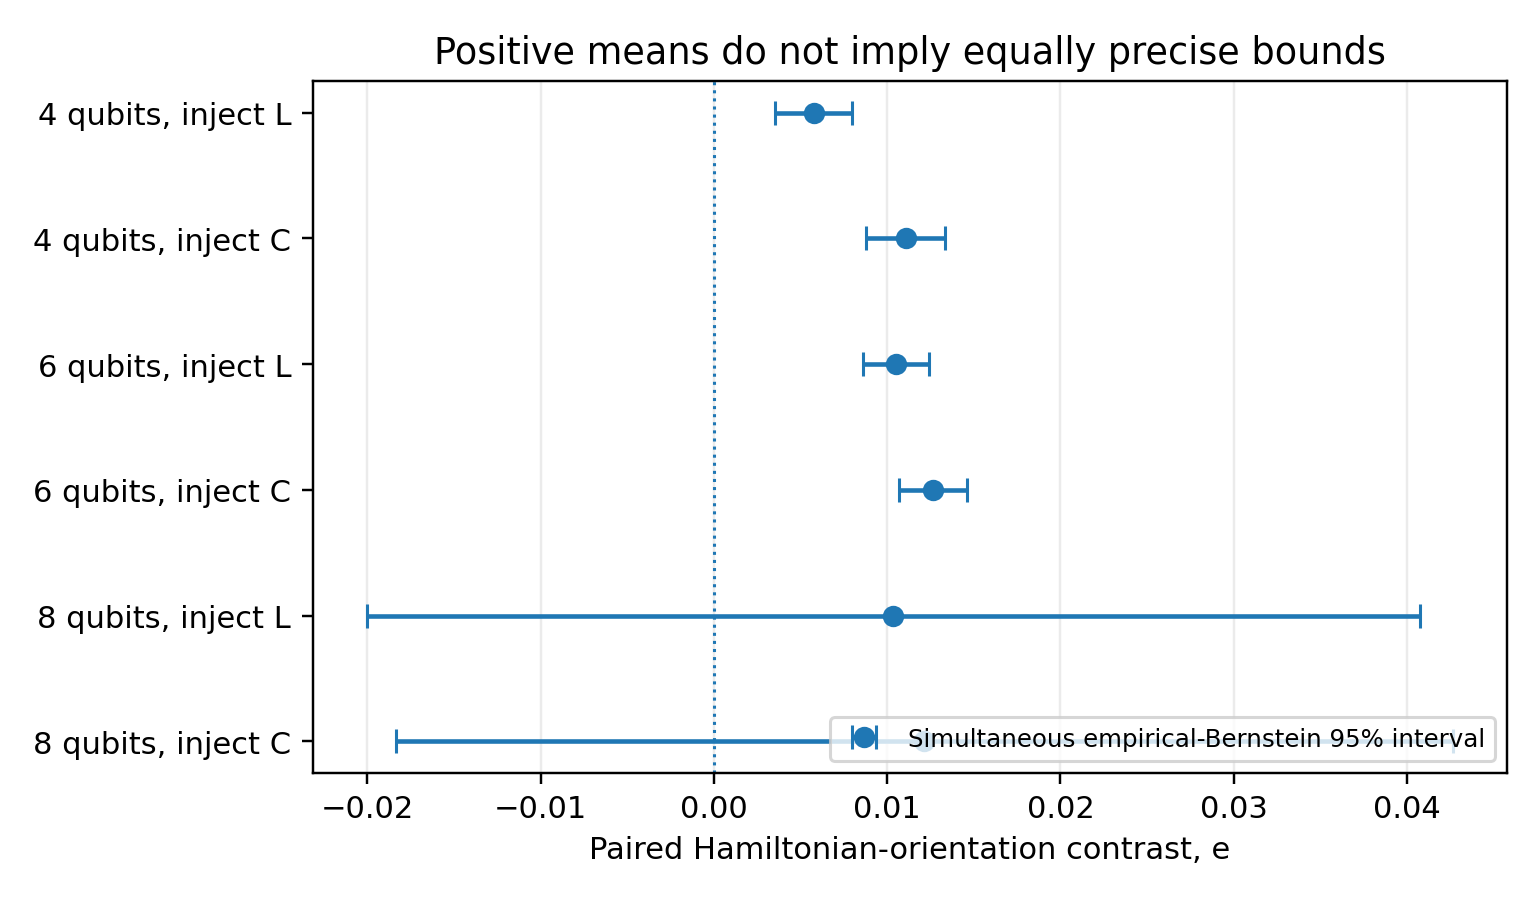
\includegraphics{../../figures/factorial_intervals.png}

\textbf{Figure 4. Different uncertainty methods answer the same six
factorial targets. Normal intervals are approximations; the displayed
Bernstein intervals use the stated finite-sample assumptions and
six-target coverage. These are not confidence intervals for AIU or
emergent spacetime.}

\end{minipage}\par\medskip

\subsubsection{9.4 What the extension
identifies}\label{what-the-extension-identifies}

The intervention changes the whole Hamiltonian's orientation relative to
fixed preparation and access. Its spectrum is unchanged, but the
prepared energy distribution and detailed state-dynamics relations need
not be. Thus the contrast supports a specified model intervention, not a
pure effect of locality with all other relevant properties held
constant. A third independent circuit frame W has intermediate supplied
mean outcomes; there is no theorem that it must be neutral or
intermediate.

The small nonzero interaction between injection and dynamics also means
that a unique additive attribution to an injection mechanism and a
locality mechanism is not supplied. A regression of z on its initial gap
contains an algebraic minus-one-half term by definition. Such regression
is descriptive unless additional assumptions identify the mechanism; an
intercept at zero gap is not by itself proof of frame selection.

Lieb-Robinson bounds constrain propagation for appropriately local
interactions. They do not imply the observed sign of the
average-readability intervention. Both Hamiltonians are related by a
fixed-depth local circuit, which enlarges native support only by a
bounded amount. Distinguishing this explanation from other finite-family
effects requires an independently chosen response or intervention test.

\subsubsection{9.5 Reproduction boundary}\label{reproduction-boundary}

The original pre-execution plan, configuration, code and receipt remain
immutable. Supplied review predictions, including the failed near-zero
factorial prediction, are preserved. Re-execution is not external
scientific replication and does not verify the claimed chronological
creation of those review predictions. Selected factorial trajectories
were checked with exponential action and full-density-matrix partial
traces rather than the source's spectral/Bloch implementation; the
separate check report records its actual scope.

New commands and numerical assumptions are in the Supplementary
Information. The archive includes the original source-off trajectories,
new factorial unit summaries, all three supplied review scripts,
reference outputs and fresh replay outputs. No outside correspondence,
peer review or publication was performed.

\subsection{10. Secondary-analysis
sources}\label{secondary-analysis-sources}

The exact binomial calculation follows directly from independent
equiprobable signs under the null. See Penn State STAT 415, Section
20.1, \emph{The Sign Test for a Median}, for the median interpretation
and its distinction from a mean test. The original contrast data, rather
than only the rounded summary, are used by
\nolinkurl{code/analyze_review_additions.py}. It also reconstructs each
unit contrast from raw trajectories and writes the four-row sign tests,
transport-encoding curves and initial-eligibility diagnostics. These are
analyses of the same pilot, not independent replication.

The mathematical source of the range-only confidence bound remains
Hoeffding (1963), cited in the methods paper. Holm adjustment is applied
to the four disclosed post hoc sign tests; it does not make them
predeclared. No new participant, cosmological or quantum-device data
were collected.

Holm, S. (1979). A simple sequentially rejective multiple test
procedure. Scandinavian Journal of Statistics 6(2), 65-70.
\url{https://www.jstor.org/stable/4615733}

Penn State STAT 415. Section 20.1, The Sign Test for a Median.
\url{https://online.stat.psu.edu/stat415/lesson/20/20.1}

Maurer, A., and Pontil, M. (2009). Empirical Bernstein Bounds and Sample
Variance Penalization. COLT 2009. \url{https://arxiv.org/abs/0907.3740}

\end{document}
